\documentclass[
	a4paper, % Paper size, use either a4paper or letterpaper
	10pt, % Default font size, can also use 11pt or 12pt, although this is not recommended
	unnumberedsections, % Comment to enable section numbering
	twoside, % Two side traditional mode where headers and footers change between odd and even pages, comment this option to make them fixed
]{LTJournalArticle}
\usepackage{graphicx} % Required to insert images
\usepackage{listings} % Required for inserting code snippets
\usepackage{biblatex}

\usepackage{amsmath}
\usepackage{color}
\usepackage{hyperref}

\bibliography{report.bib}

\setcounter{page}{1} % Set the starting page number

%----------------------------------------------------------------------------------------
%	TITLE SECTION
%----------------------------------------------------------------------------------------

\title{F1 Simulation: Mixed Reality Experience}
\author{Atit Kharel}

% Affiliations are output in the \date{} command
\date{\footnotesize Department of Computer Science, \\
University of Arkansas at Little Rock}


% Full-width abstract
\renewcommand{\maketitlehookd}{%
\begin{abstract}
This report details the development of an immersive Formula 1 (F1) race simulation using Unity and data from the OpenF1 API. The project leverages mixed reality (MR) technology to provide a unique, interactive 
experience, where users can observe and interact with F1 races through Head Mounted Displays (HMDs). By utilizing data on tracks, cars, drivers, and race events, the simulation dynamically represents past races. 
The project also integrates user interactions through hand tracking and raycasting, enabling intuitive control of the simulation. This report discusses work flow of the simulation, a critial analysis of the current implementation,
along with potential improvements and enhancements, to further enhance the simulation's realism and user experience. The project showcases the potential of integrating real-world data with MR technology to create engaging and immersive experiences for 
users, which can also be leveraged to enhance data visualization and analysis across various fields.
\end{abstract}

}

%----------------------------------------------------------------------------------------

\begin{document}
\definecolor{codegreen}{rgb}{0,0.6,0}
\definecolor{codegray}{rgb}{0.5,0.5,0.5}
\definecolor{codepurple}{rgb}{0.58,0,0.82}
\definecolor{backcolour}{rgb}{0.95,0.95,0.92}

\lstdefinestyle{codestyle}{
    backgroundcolor=\color{backcolour},   
    commentstyle=\color{codegreen},
    keywordstyle=\color{magenta},
    numberstyle=\tiny\color{codegray},
    stringstyle=\color{codepurple},
    basicstyle=\ttfamily\footnotesize,
    breakatwhitespace=false,
    breaklines=true,
    captionpos=b,
    keepspaces=true,
    numbers=left,                   
    numbersep=5pt,               
    showspaces=false,
    showstringspaces=false,
    showtabs=false,                  
    tabsize=2,
    language=[Sharp]C,
}

\lstset{style=codestyle}

\maketitle

\section{Introduction}
The objective of the F1 Simulation project is to integrate real-world data from the OpenF1 API \autocite{godefroy_openf1} into a mixed reality (MR) environment on HMDs 
like the Oculus Quest 3 \autocite{oculus_quest_3}. The aim is to simulate a real-time Formula 1 race, allowing users to interact with the race virtually and view it in an 
MR setting. The Unity engine was chosen as the platform for development due to its support for multiple headsets and its robust 3D rendering capabilities.

\section{Technologies}
\subsection{Unity}
Unity was used as the main development environment, providing the necessary tools for building 3D environments and integrating virtual objects into a mixed-reality experience. 
The engine's C\# scripting capabilities were used to implement the simulation's logic and interactions.

\subsection{OpenF1 API}
The OpenF1 API is an open-source platform that provides real-time or historical data on Formula 1 race events, drivers, teams, and tracks. These data were used to populate the 
simulation with accurate information to visualize the drivers, cars, and track.

\subsection{Meta All-In-One XR Plugin}
The Meta All-In-One XR is a plugin provided by Meta that enables developers to create immersive experiences in both virtual reality (VR) and mixed reality (MR). The plugin offers 
features such as hand tracking, spatial mapping, hand tracking, which were utilized in the project.

\subsection{Oculus Quest 3}
The Oculus Quest 3 is a standalone VR headset that provides a wireless and untethered experience. The device was used to test the MR simulation, using the device's hand tracking 
and spatial mapping capabilities to enhance the development process.

\section{Project Components}
\subsection{Data Collection and Processing}
The project communicates with multiple endpoints of the OpenF1 API to fetch data on tracks, driver details, car telemetry, and their location on the track using coroutine in Unity. 
The fetched data is processed (stored and sorted accendingly by date/time) for each data entry to ensure the simulation runs in chronological order. The data is then used to populate 
the simulation by spawning new car for each driver and updating their position and telemetry.

To update the data for simulation, a virtual countdown timer is used to simulate the data updates. We take the time difference between the current time and the time of the next data 
entry to update the simulation and interpolate the car position to avoid sudden jumps for inconsistent data.

Each driver can have around 22,000 data entries for each category depending on track size, with each data entry having their own timestamp. The data is fetched and processed in 
real-time to simulate which makes it usable even in live race senarios not limiting to historical race simulations.

\subsection{Environment and UI}
The simulation starts with a 3d plane representing the track, with 3D models of cars on the track. Each car also has a name tag with the driver's acronym for identification. 
The user interface (UI) [Figure \ref{fig:main_ui_unity}] has 3 main components: a plane with track's image, a leaderboard on the left (with position, name and interval from leader), 
and a driver telemetry panel on the right (with speed, gear, RPM, and throttle/brake input). The virtual clock for the simulation is displayed at the top of the UI, showing the current time in the simulation.

% add figure 
\begin{figure}[h] % Single column figure
	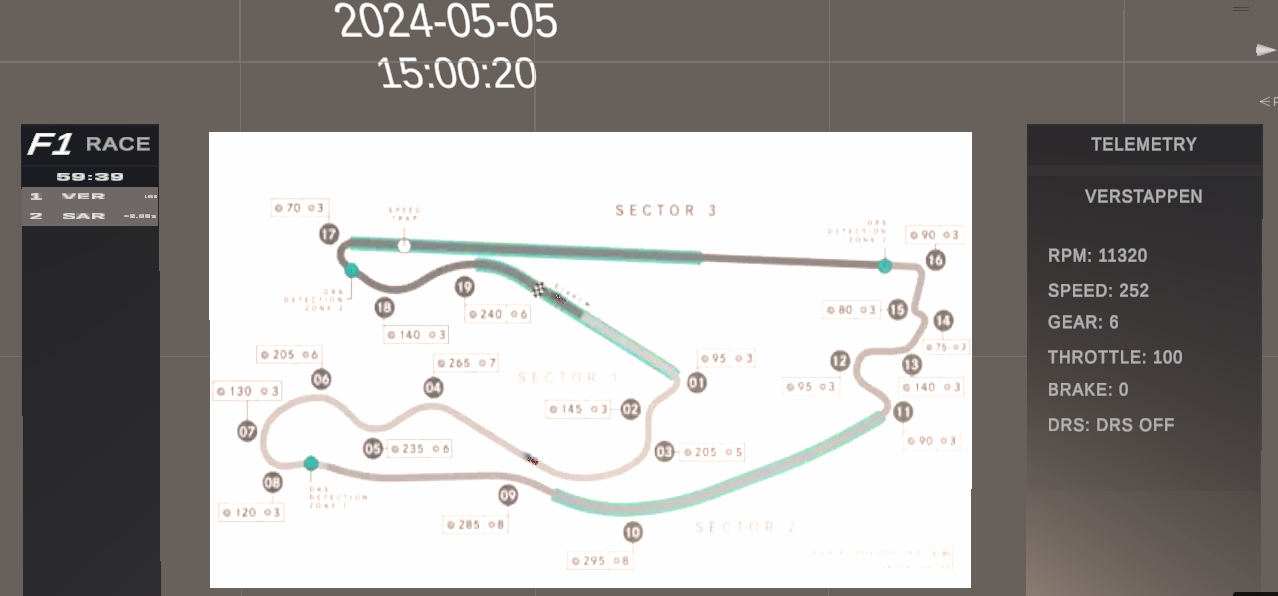
\includegraphics[width=\linewidth]{main_ui.png}
	\caption{Main UI of the F1 Simulation}
    \label{fig:main_ui_unity}
\end{figure}

For controlling the simulation, the user can use a sim control UI [Figure \ref{fig:sim_controller_ui}], toggled by pressing 'X' button on the left controller.
The Control UI allows the user to start, pause, reset, increse or decrease the simulation speed. Both controller and hand tracking can be used to interact with the UI.

\begin{figure}[h] % Single column figure
	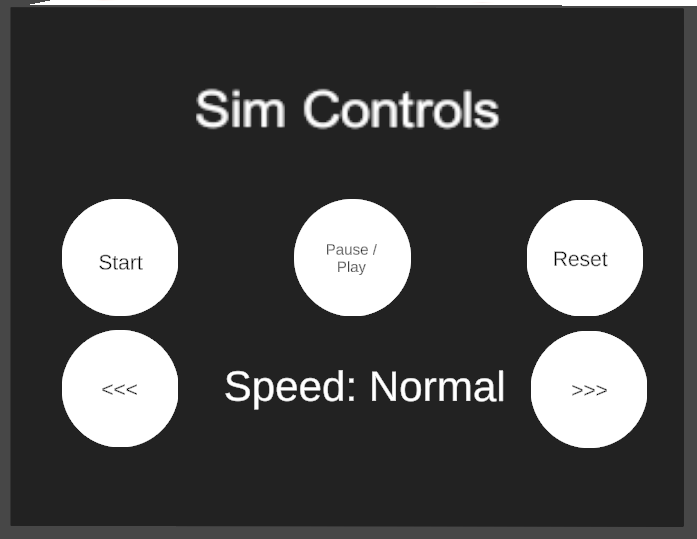
\includegraphics[width=\linewidth]{sim_controller_ui.png}
	\caption{Simulation Controller UI}
    \label{fig:sim_controller_ui}
\end{figure}

\subsection{Car Simulation}

To update the car's position in simulation, the system uses a method that receives a driver's number and a list of track data entries (containing time, position and telemetry data). 
The method then uses binary search to find the correct interval of data points that surround the current simulation time. These two points, referred to as \verb|prevData| or $\mathbf{p}_{\text{prev}}$ 
and \verb|nextData| or $\mathbf{p}_{\text{next}}$, are the closest time-stamped positions before and after the current time. If valid previous and next points are found, the car's position and rotation is updated by interpolating between these two data points. This results in smooth movement and rotation of the car between the two data points.

\subsubsection{Position Interpolation}
Given two data points, the previous position $\mathbf{p}_{\text{prev}} = (x_{\text{prev}}, y_{\text{prev}})$ and the next position $\mathbf{p}_{\text{next}} = (x_{\text{next}}, y_{\text{next}})$, 
the interpolation factor $t$ is calculated as:

\[
t = \frac{\Delta t_{\text{simulated}}}{\Delta t_{\text{interval}}} = \frac{T_{\text{simulated}} - T_{\text{prev}}}{T_{\text{next}} - T_{\text{prev}}}
\]

where $T_{\text{simulated}}$ is the current simulation time, and $T_{\text{prev}}$ and $T_{\text{next}}$ are the timestamps of the previous and next data points, respectively.

The interpolated position $\mathbf{p}(t)$ is given by:

\[
\mathbf{p}(t) = (1 - t) \mathbf{p}_{\text{prev}} + t \mathbf{p}_{\text{next}}
\]

Expanding into components:

\[
x(t) = (1 - t) x_{\text{prev}} + t x_{\text{next}}, \quad y(t) = (1 - t) y_{\text{prev}} + t y_{\text{next}}
\]

\subsubsection{Rotation Interpolation}
The car’s angle $\theta$ between the previous and next positions is calculated as:

\[
\theta = \arctan \left( \frac{\Delta x}{\Delta y} \right) = \arctan \left( \frac{x_{\text{next}} - x_{\text{prev}}}{y_{\text{next}} - y_{\text{prev}}} \right)
\]

\textbf{Note:} only two coordinates are used for interpolation as the car's elevation data is not considered in this project, but it is provided in the OpenF1 API data.

\subsubsection{Implementation}

The interpolation is achieved in Unity by using the \verb|Vector3.Lerp| function for position \& \verb|Mathf.Atan2| and \verb|Quaternion.Slerp| for angle and rotation. 
[Listing \ref{lst:interpolation}] shows the C\# code that implements the described method.

\begin{lstlisting}[caption=Interpolation of Car Position and Rotation, label=lst:interpolation]
    private void InterpolatePosition(int driverNumber, TrackData prevData, TrackData nextData)
    {
        float timeBetween = (float)(DateTime.Parse(nextData.date) - DateTime.Parse(prevData.date)).TotalSeconds;
        float timeSincePrev = (float)(simulatedTime - DateTime.Parse(prevData.date)).TotalSeconds;
        float t = Mathf.Clamp01(timeSincePrev / timeBetween);

        // Interpolate position
        Vector3 prevPosition = new Vector3(prevData.x, 0, prevData.y);
        Vector3 nextPosition = new Vector3(nextData.x, 0, nextData.y);
        Vector3 interpolatedPosition = Vector3.Lerp(prevPosition, nextPosition, t);
        carModels[driverNumber].transform.localPosition = interpolatedPosition;

        // Interpolate rotation
        float angle = Mathf.Atan2(nextPosition.x - prevPosition.x, nextPosition.z - prevPosition.z) * Mathf.Rad2Deg;
        carModels[driverNumber].transform.localRotation = Quaternion.Slerp(carModels[driverNumber].transform.localRotation, Quaternion.Euler(0, angle, 0), t);
    }
\end{lstlisting}

\subsection{Leaderboard and Telemetry}
The leaderboard on the left is updated based on the data's timestamp, with the leaderboard showing the driver's position, name, and interval from the leader. The telemetry panel on the right displays the driver's speed, gear, RPM, and throttle/brake input which is updated similarly to the car's position as both the data is from the same data entry.

\subsection{Interactions}
For the sim control UI, the user needs controller input to toggle the UI and interact with the buttons. Other than that, the simulation supports both controller and hand tracking for interactions. The user is able to grab the main track UI and move or rotate it using the controller or hand tracking. Users can use two hands to grab the track and scale it to zoom in or out.

\section{Critical Analysis}

\subsection{Interaction Enhancements}
The simulation's current interaction model is confusing and lacks intuitiveness. It can be enhanced by adding more features like gesture recognition, voice commands, or gaze-based interactions. These features can provide a more intuitive and immersive experience for the user, allowing them to control the simulation more naturally.

\subsection{Environment Awareness}
The simulation's environment awareness can be improved by integrating spatial mapping. This can help the simulation adapt to the user's physical environment, providing a more realistic and immersive experience. Spatial mapping can also be used to create more interactive elements in the simulation, such as placing the track in the user's physical space like a tabletop, floor or wall.
\subsection{Performance Optimization}
The simulation currently loads all the data first and then processes it, which can lead to performance issues with large datasets. To optimize performance, the simulation can be modified to load and process data in chunks or on-demand, reducing the initial load time and memory usage.

\subsection{Local Data Storage}
The simulation currently fetches data from multiple OpenF1 API endpoints, which can lead to network latency and data synchronization issues. To address this, we can setup a local database to store the data and update it periodically to ensure the simulation runs smoothly and efficiently without relying on external APIs.

\section{Improvements and Future Work}
The F1 Simulation project has the potential for further improvements and enhancements to provide a more engaging and immersive experience for users. Some of the key areas for improvement include:
\subsection{Multiplayer Support}
Adding multiplayer support to the simulation can enhance the user experience by allowing multiple users to interact with the simulation simultaneously. 

\subsection{Real-time Data Updates}
The simulation can be enhanced to support real-time data updates, allowing users to view live Formula 1 races not limited to historical races.

\subsection{Driver Performance Analysis}
The simulation can be extended to include driver performance analysis, such as lap times, sector times, and even compare driver telemetry data to identify driving patterns and strategies. This can provide valuable insights for fans, teams, and analysts.

\subsection{Weather and Track Conditions}
Taking weather data from the OpenF1 API, the simulation can be enhanced to include dynamic weather and track conditions, such as rain, fog, or changing track temperatures. This can add an extra layer of realism and challenge to the simulation.

\section{Conclusion}
The F1 Simulation project demonstrates the potential of integrating real-world data with mixed reality technology to create immersive and interactive experiences for users. By leveraging the OpenF1 API and Unity engine, the project simulates Formula 1 races introducing the concept of a digital twin, where the virtual simulation mirrors real-world race events and conditions. By utilizing this concept, the project not only provides an engaging user experience but also opens up possibilities for advanced data visualization and analysis, making it a potentially valuable tool for both entertainment and professional applications.
\printbibliography

\end{document}